\section{Supplementary results}
\label{app:extra}

\subsection{The anomaly that motivated the study}

\begin{figure}[htbp]
\centering
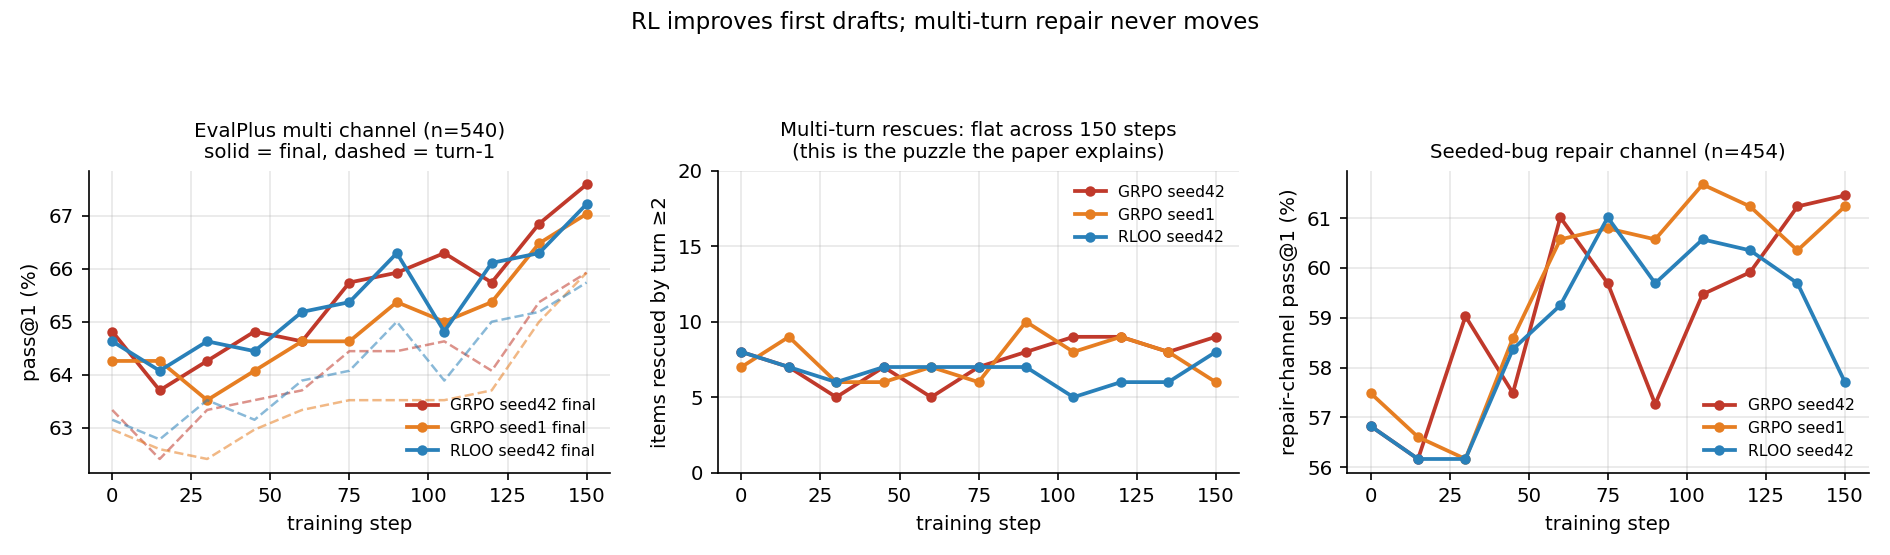
\includegraphics[width=\linewidth]{fig4_training_curves.png}
\caption{Left: pass@1 rises over 150 steps on all three runs, driven by first drafts (dashed)
rather than final answers. \textbf{Centre: the count of items rescued by turn 2 or later never
moves} --- 6--9 out of 540 from step 0 to step 150, across two algorithms and two seeds. Right:
the seeded-bug repair channel does improve, confirming the model is learning something about
fixing code; it simply never does so \emph{across turns}. \S\ref{sec:rl} shows the tool was
never successfully called in any of these runs.}
\label{fig:training_curves}
\end{figure}

\subsection{Result tables referenced from \S\ref{sec:results}}
\label{app:tables}

\begin{center}
\small
\captionof{table}{BFCL v4, first HTTP request per case. Intent columns are measured only where the parse failed.}\label{tab:bfclfunnel}
\setlength{\tabcolsep}{3.5pt}\begin{tabular}{@{}llllllll@{}}
\toprule
Arm & cases & HTTP err & first parsed & unparsed & tight & strong & weak \\
\midrule
\texttt{hermes} (documented) & 200 & 0 & \textbf{0} & 200 & 166 & 169 & 187 \\
\texttt{qwen2\_5\_coder} (repaired) & 200 & 0 & \textbf{196} & 4 & 0 & 1 & 2 \\
\bottomrule
\end{tabular}
\end{center}
\begin{center}
\small
\captionof{table}{$\tau$-bench \texttt{retail}, all 115 tasks paired across arms (none dropped).}\label{tab:tau}
\begin{tabular}{@{}lrr@{}}
\toprule
 & documented & repaired \\
\midrule
assistant turns & 1389 & 1971 \\
server-parsed calls & \textbf{0} & \textbf{636} \\
emitted but unparsed & \textbf{789} & 6 \\
tool executions / observations returned & \textbf{0} & \textbf{636} \\
\midrule
tasks entering the tool loop at all & \textbf{0} & \textbf{103} \\
tasks solved & 7 & 10 \\
\bottomrule
\end{tabular}
\end{center}
\begin{center}
\small
\captionof{table}{Same probe, items and criterion under a \emph{matched} envelope.}\label{tab:counterfactual}
\begin{tabular}{@{}lll@{}}
\toprule
Size & server-parsed & \textbf{silent fraction (tight, unparsed)} \\
\midrule
Qwen3-0.6B & 86 & \textbf{1} \\
Qwen3-1.7B & 44 & \textbf{1} \\
Qwen3-4B & 70 & \textbf{2} \\
Qwen3-8B & 97 & \textbf{0} \\
\midrule
Qwen2.5-Coder 1.5B--32B (mismatched) & 0 at every size & \textbf{0 $\to$ 4 $\to$ 21 $\to$ 36 $\to$ 80} \\
\bottomrule
\end{tabular}
\end{center}
\begin{center}
\small
\captionof{table}{Qwen2.5-Instruct under the identical mismatched configuration, with both ladders' task outcomes measured on a working executor.}\label{tab:instruct}\label{tab:turn1}
\setlength{\tabcolsep}{3.5pt}\begin{tabular}{@{}llll|ll|lll@{}}
\toprule
& \multicolumn{3}{c|}{Instruct, emitted} & \multicolumn{2}{c|}{Coder} & \multicolumn{3}{c}{Instruct} \\
Size & parsed & \textbf{tight} & weak & parsed & turn-1 = final & turn-1 & final & \textbf{rescued} \\
\midrule
1.5B & 1 & 0 & 7 & 0 & 31 & 13 & 13 & \textbf{0} \\
3B & 11 & 56 & 2 & 0 & 37 & 14 & 17 & \textbf{+3} \\
7B & 63 & 21 & 0 & 0 & 53 & 34 & 40 & \textbf{+6} \\
14B & 77 & 19 & 0 & 0 & 53 & 38 & 52 & \textbf{+14} \\
\textbf{32B} & \textbf{88} & 8 & 0 & 0 & 68 & 42 & 65 & \textbf{+23} \\
\bottomrule
\end{tabular}
\end{center}
\begin{center}
\small
\captionof{table}{Llama-3.1-8B arms, paired on the same 100 items.}\label{tab:llama_arms}
\begin{tabular}{@{}llllll@{}}
\toprule
Arm & Calls issued & Wrong-tool & Executed & Turn-1 & Final \\
\midrule
terse (parser only) & 97 & 23 & 74 & 34 & 49 \\
+ official template & 95 & 22 & 73 & 33 & 44 \\
+ official template \textbf{+ \texttt{strict}} & 98 & \textbf{0} & \textbf{97} & \textbf{46} & \textbf{61} \\
ReAct (reference) & 98 & 0 & 97 & \textbf{61} & 80 \\
\bottomrule
\end{tabular}
\end{center}
\begin{center}
\small
\captionof{table}{Decomposing the ReAct--FC gap on Llama, paired McNemar.}\label{tab:decomposition}
\begin{tabular}{@{}llll@{}}
\toprule
Comparison & b/c & \emph{p} & Attributable to \\
\midrule
terse-FC $\to$ strict-FC (49 $\to$ 61) & 15/3 & \textbf{0.0075} & \textbf{interface repair, +12} \\
strict-FC $\to$ ReAct (61 $\to$ 80) & 27/8 & \textbf{0.0019} & \textbf{protocol, +19} \\
terse-FC $\to$ ReAct (49 $\to$ 80) & 38/7 & 3.1e-06 & both, +31 \\
\bottomrule
\end{tabular}
\end{center}
\begin{center}
\small
\captionof{table}{Repair loop on Qwen2.5-Coder-7B, \texttt{tool\_choice: auto} fixed, changing only the adapter.}\label{tab:repair}
\begin{tabular}{@{}lllllll@{}}
\toprule
Arm & Parsed & Mean turns & $\geq$2 turns & Turn-1 & Final & Rescued \\
\midrule
ReAct & 95 & 1.92 & 40 & 57 & \textbf{74} & 17 \\
FC + hermes & \textbf{0} & 0.96 & \textbf{0} & 53 & 53 & \textbf{0} \\
FC + dedicated adapter & \textbf{84} & 1.82 & \textbf{37} & 53 & \textbf{62} & \textbf{9} \\
\bottomrule
\end{tabular}
\end{center}
\begin{center}
\small
\captionof{table}{RL training rollouts, matched in model, data, hyper-parameters, seed and prompt strength.}\label{tab:training}
\begin{tabular}{@{}lllll@{}}
\toprule
Arm & Steps & \texttt{num\_turns/mean} & Tool time & Tool calls / rollout \\
\midrule
FC (\texttt{tool\_agent} + hermes) & 10 & \textbf{2.000} (constant) & \textbf{0.00 s} & \textbf{0.000} \\
ReAct (\texttt{react\_agent}) & 3 & 5.883 & 12.21 s & \textbf{2.052} \\
\bottomrule
\end{tabular}
\end{center}

\subsection{Offline re-parse matrix and failure-layer decomposition}
\label{app:reparse}

To exclude ``your extractor is simply better than \texttt{hermes}'', we re-parsed the
\emph{same stored bytes} under four rules (\texttt{analysis/reparse\_matrix.py}, no GPU).

\begin{center}
\small
\captionof{table}{The same bytes, re-parsed offline under four rules. Where the server already parsed a call, \texttt{content} is empty and offline replay has nothing to read; those cells are N/A rather than zero. The gap is a parser mismatch, not a claim that no parser could have read the output.}\label{tab:reparse}
\begin{tabular}{@{}llllll@{}}
\toprule
Arm (server-parsed = 0) & server & hermes replay & \texttt{<tools>} replay & bare JSON & tight \\
\midrule
Qwen-1.5B & 0 & 0 & 0 & 0 & 0 \\
Qwen-3B & 0 & 0 & 0 & 5 & 4 \\
Qwen-7B & 0 & 0 & 0 & 22 & 21 \\
Qwen-14B & 0 & 0 & 0 & 42 & 36 \\
Qwen-32B & 0 & \textbf{0} & 0 & \textbf{100} & \textbf{80} \\
\bottomrule
\end{tabular}
\end{center}

The \texttt{hermes} column is zero at every scale: the model never produces that format. The
bare-JSON and tight columns are not: the calls exist, and their difference from the server
column is precisely what the format mismatch removes. For arms where the server \emph{did}
parse, offline content-only re-parsing is \textbf{undefined, not zero} --- a successful parse
moves the call into \texttt{tool\_calls} and leaves \texttt{content} empty.

Replaying vLLM~0.27.1's \texttt{hermes} extractor line for line over the stored bytes
(\texttt{analysis/failure\_layer.py}) separates the layer at which each item is lost: no
\texttt{<tool\_call>} envelope at all; envelope present but the JSON payload malformed; payload
well-formed and rejected only because \texttt{json.loads} does not tolerate trailing text in the
capture; or a genuine parser loss, meaning the replay succeeds where the server did not.

\begin{center}
\small
\captionof{table}{Where the unparsed items are lost. Coder fails entirely at the envelope; Instruct reaches the envelope and fails at the payload. \textbf{Genuine parser loss is zero in every arm} --- and across all 4254 de-duplicated first turns in the archive.}\label{tab:layer}
\begin{tabular}{@{}lllll@{}}
\toprule
Arm & no envelope & payload malformed & strictness only & \textbf{parser loss} \\
\midrule
Coder 1.5B--32B (all sizes) & 100 & 0 & 0 & \textbf{0} \\
Instruct 1.5B & 93 & 6 & 0 & \textbf{0} \\
Instruct 3B & 22 & 41 & 26 & \textbf{0} \\
Instruct 7B & 3 & 33 & 1 & \textbf{0} \\
Instruct 14B & 13 & 6 & 4 & \textbf{0} \\
Instruct 32B & 1 & 9 & 2 & \textbf{0} \\
\bottomrule
\end{tabular}
\end{center}

The two ladders fail at different layers: Coder emits a well-formed bare call and never the
envelope, so \texttt{hermes} not seeing it is \emph{correct behaviour}; Instruct emits the
envelope and then breaks the JSON, almost always by embedding Python whose docstring quotes or
raw newlines are left unescaped inside the \texttt{code} string. And \textbf{in no arm --- across
the whole archive --- did the server fail to parse a call that its own extractor would have
accepted.} ``Censoring'' throughout this paper therefore means \emph{the attempt never reaches
the parser in a form it is defined to accept}, not \emph{the parser discards valid calls}.

\subsection{BFCL: gating and the full reproduction record}
\label{app:bfcl}

Each arm passes a two-case end-to-end smoke test before its full run, and a run is rejected
unless the result count, the score file's \texttt{total\_count} and the number of distinct case
ids in the recording proxy all agree at 200 with zero HTTP errors. Both arms run at \texttt{max\_model\_len = 16384}, \texttt{temperature = 0} and inference seed
0, on cases drawn at manifest seed 20260901. Registration of BFCL's OpenAI
handler happens in memory at import time, so \texttt{bfcl\_eval}'s own files are left
byte-identical; a recording proxy sits between benchmark and server and logs every request.

We ran the pair twice. The \texttt{hermes} arm is identical across runs in every column: 0/200
parsed, 166 tight, 480 requests, 0 errors. The repaired arm moves by one case between runs ---
\textbf{197 versus 196} first parsed, \textbf{99 versus 98} executed --- while success is 19 in
both. Greedy decoding does not make vLLM bitwise deterministic across differing batch
compositions, and this arm runs eight threads through a multi-turn executor, so we report its
intermediate funnel columns as $\pm1$ rather than exact.

\begin{center}
\small
\captionof{table}{BFCL \texttt{multi\_turn\_base}, n = 100, joined to the HTTP trace by case id.}\label{tab:bfcl5}
\begin{tabular}{@{}lllllll@{}}
\toprule
Arm & tight (unparsed) & first parsed & any parsed & executed & \textbf{success} & rescued \\
\midrule
\texttt{hermes} & 69 & 0 & 0 & 0 & \textbf{0} & 0 \\
\texttt{qwen2\_5\_coder} & 0 & 97 & 98 & 98 & \textbf{19} & 0 \\
\bottomrule
\end{tabular}
\end{center}

\begin{center}
\small
\captionof{table}{Two quantified failure layers; the full four-family table is Table~\ref{tab:taxonomy_full}.}\label{tab:taxonomy}
\begin{tabular}{@{}p{.14\linewidth}p{.10\linewidth}p{.25\linewidth}p{.22\linewidth}p{\dimexpr.29\linewidth-8\tabcolsep\relax}@{}}
\toprule
Family & Layer & Symptom & Detectable in advance? & Remedy \\
\midrule
Qwen2.5-Coder & parser & emits a fenced JSON block, not \texttt{<tool\_call>}
  & $\times$ template check \textbf{false-positives} & dedicated adapter \\
Llama-3.1-8B & schema & calls the \emph{task function} as a tool (23\%)
  & $\times$ requires argument inspection & \texttt{strict: true} \\
\bottomrule
\end{tabular}
\end{center}

\subsection{The full four-family taxonomy}
\label{app:taxonomy}

\begin{center}
\small
\captionof{table}{Four families, four layers. Only Mistral's failure announces itself.}\label{tab:taxonomy_full}
\begin{tabular}{@{}p{.14\linewidth}p{.10\linewidth}p{.25\linewidth}p{.22\linewidth}p{\dimexpr.29\linewidth-8\tabcolsep\relax}@{}}
\toprule
Family & Layer & Symptom & Detectable in advance? & Remedy \\
\midrule
DeepSeek-Coder & template & chat template never injects tools
  & $\checkmark$ template inspection & none \\
Qwen2.5-Coder & parser & emits a fenced JSON block, not \texttt{<tool\_call>}
  & $\times$ template check \textbf{false-positives} & dedicated adapter \\
Llama-3.1-8B & schema & calls the \emph{task function} as a tool (23\%)
  & $\times$ requires argument inspection & \texttt{strict: true} \\
Mistral-7B-v0.3 & token & repeats \texttt{[TOOL\_CALLS]} $\to$ HTTP 400
  & $\sim$ errors, but only sometimes & \textbf{none found} \\
\bottomrule
\end{tabular}
\end{center}

\begin{figure}[htbp]
\centering
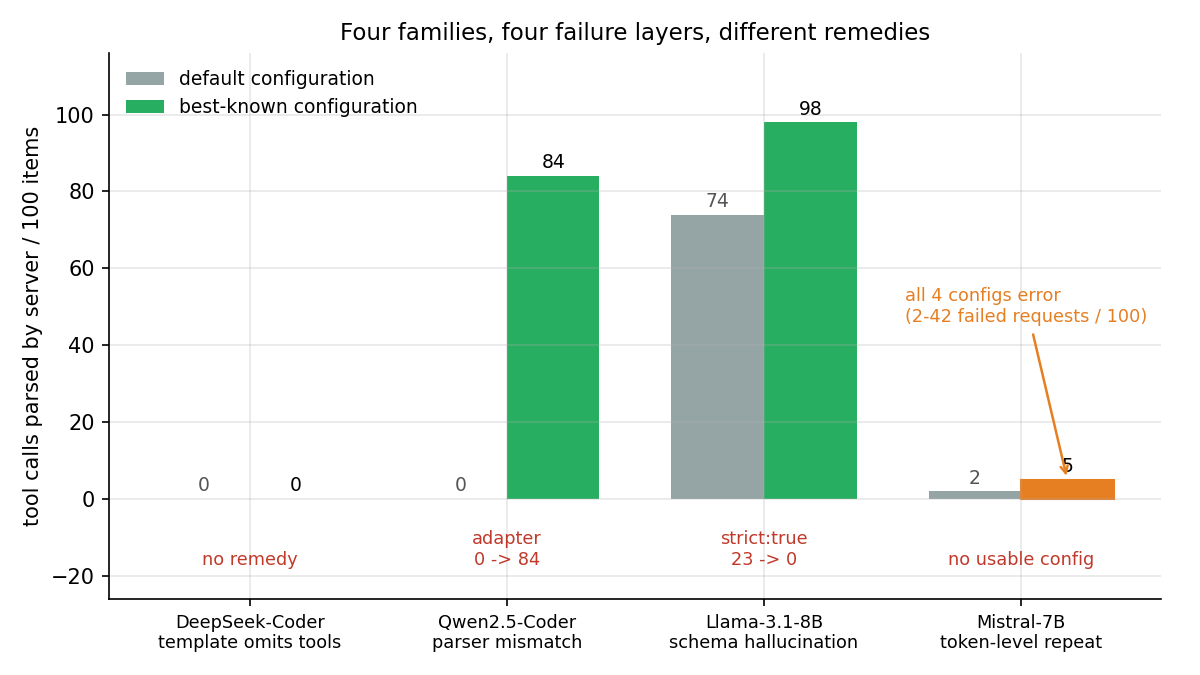
\includegraphics[width=\linewidth]{fig2_family_taxonomy.png}
\caption{The same four failures, quantified. Grey is the configuration a reader arrives at by
following the documentation; green is the best configuration we found. Mistral never produces an
error-free run under any of four configurations, so its bars are not comparable with the others
and are drawn in orange.}
\label{fig:taxonomy}
\end{figure}

\begin{figure}[htbp]
\centering

\includegraphics[width=0.72\linewidth]{fig1_intent_parse_gap.png}
\caption{Within-family observation under the mismatched interface. Across the five
Qwen2.5-Coder checkpoints, the server parses zero calls while tight-classified emissions
rise to 80/100 at 32B (approximately 72 after calibration with tight-stratum precision
0.900, assuming transfer across sizes; Appendix~\ref{app:humanval}). Same data as
Table~\ref{tab:scale}.}
\label{fig:gap}
\end{figure}

\subsection{Main table under unified configuration}
\label{sec:maintable_full}

\begin{center}
\small
\setlength{\tabcolsep}{4pt}
\captionof{table}{All arms genuinely at \texttt{max\_tokens}=2048, one shared 100-item set, \texttt{temperature}=0. Mistral has no admissible FC arm: all four configurations produce request errors, so no pass rate and no \emph{p}-value are computed.}\label{tab:main}
\setlength{\tabcolsep}{3.5pt}\begin{tabular}{@{}llllllll@{}}
\toprule
Model & \multicolumn{2}{c}{ReAct} & \multicolumn{2}{c}{FC} & b/c & \emph{p} & FC arm \\
\cmidrule(lr){2-3}\cmidrule(lr){4-5}
 & turn-1 & final & turn-1 & final & & & \\
\midrule
Llama-3.1-8B & 61 & \textbf{80} & 46 & 61 & 27/8 & \textbf{0.0019} & official tmpl.\ + \texttt{strict} \\
Qwen2.5-Coder-7B & 57 & \textbf{74} & 53 & 62 & 17/5 & \textbf{0.0169} & dedicated adapter \\
Mistral-7B-v0.3 & 26 & 33 & N/A & N/A & N/A & N/A & --- \\
\bottomrule
\end{tabular}
\end{center}

\subsection{The four Llama controls, tabulated}

\begin{center}
\small
\captionof{table}{Four single-variable controls on Llama-3.1-8B's 23\% wrong-tool rate. The first three rejected their alternative explanations and pointed at the model; the fourth found the actual cause and withdrew that conclusion.}\label{tab:controls}
\begin{tabular}{@{}p{.27\linewidth}p{.21\linewidth}p{.27\linewidth}p{\dimexpr.25\linewidth-6\tabcolsep\relax}@{}}
\toprule
Alternative explanation & Control & Empty-argument rate & Verdict \\
\midrule
schema lacks a parameter description & rich vs terse & 23 $\to$ 22 (\emph{p}=1.000) & rejected \\
ReAct merely adds a reasoning step & FC + Thought scaffold & 23 $\to$ \textbf{59} (\emph{p}\textless0.001, \textbf{worse}) & rejected \\
server not configured per documentation & + official chat template & 23 $\to$ 22 (1/0 discordance, \emph{p}=1.000) & rejected \\
\textbf{schema constraint not enabled} & \textbf{+ \texttt{strict: true} on official template} & \textbf{22 $\to$ 0 (22/0, \emph{p}=4.77$\times10^{-7}$)} & \textbf{accepted} \\
\bottomrule
\end{tabular}
\end{center}

\subsection{Conditioning on a successful parse, and access vs.\ use of feedback}
\label{app:conditioned}

\begin{center}
\small
\captionof{table}{Conditioning on items where both protocols parsed successfully. The residual protocol gap holds on Llama and does not reach significance on Qwen --- the honest reading is one family out of two, not a general law.}\label{tab:conditioned}
\begin{tabular}{@{}llllll@{}}
\toprule
Family & Items both parsed & ReAct & FC & b/c & \emph{p} \\
\midrule
Qwen2.5-Coder-7B & 83 & 63 & 56 & 11/4 & \textbf{0.119 (n.s.)} \\
Llama-3.1-8B & 96 & 78 & 60 & 25/7 & \textbf{0.0021} \\
\bottomrule
\end{tabular}
\end{center}

\begin{center}
\small
\captionof{table}{Repair success given that feedback was actually received. Conditioned this way the two protocols are much closer, which locates the gap in \emph{how often feedback arrives} rather than in what the model does with it. On Qwen this difference is within the non-significant band above, so we state it as an observation, not a result.}\label{tab:given_feedback}
\begin{tabular}{@{}llll@{}}
\toprule
Arm & Reached turn $\geq$2 & Rescued & Repair success given feedback \\
\midrule
ReAct & 40 & 17 & \textbf{42\%} \\
FC + adapter & 37 & 9 & \textbf{24\%} \\
FC + hermes & \textbf{0} & \textbf{0} & undefined \\
\bottomrule
\end{tabular}
\end{center}

\textbf{Adapters are not a universal switch.} The same adapter recovers 84/100 at 7B and
\textbf{1/100 at 3B}: the 3B checkpoint ignores the \texttt{<tools>} few-shot entirely (zero
\texttt{<tools>} tags in 100 items, 99 direct code) while still solving the task at a comparable
rate (final 53). Adapter effectiveness is non-monotonic in scale, reinforcing the per-checkpoint
claim of \S\ref{sec:families}. The dedicated solution also changes parser, chat template and
few-shot simultaneously; we additionally rewrote the template's few-shot examples, which
originally invoked \texttt{get\_weather} --- a tool absent from our schema, which would have
induced calls to a non-existent tool and inflated both initiation and empty-argument counts.
Original and modified hashes are recorded.

\subsection{Pressure on a broken interface makes things worse}
\label{sec:pressure}

Two independent controls point the same way. Adding a reasoning scaffold to FC raised role
confusion from 23 to \textbf{59} (\S\ref{sec:llama}). Replacing the optional tool instruction
with a mandatory one on Qwen2.5-Coder-1.5B moved parser-accepted calls not at all --- still
0/100 --- while final pass fell from \textbf{31 to 15} and unparsable outputs rose from
${\sim}0$ to 46/100. Neither intervention touches the interface, and both make the observable
outcome worse. \textbf{When an agent appears reluctant to use tools, strengthening the
instruction is the cheapest thing to try and the most likely to mislead} --- it can degrade task
performance while leaving the tool-call count at zero, which looks like a model that is both
unwilling \emph{and} incapable.

\begin{center}
\small
\captionof{table}{Probe replication on the 1.5B model actually being trained, same mandatory prompt (n=100). Not one output names \texttt{run\_tests}, so at this scale the missing calls are not a parser mismatch --- there was nothing well-formed to censor.}\label{tab:probe_categories}
\begin{tabular}{@{}lll@{}}
\toprule
Category & n & \% \\
\midrule
wrong name, \texttt{arguments} carry complete code & \textbf{0} & 0\% \\
wrong name, \texttt{arguments} are the task function's parameters & \textbf{36} & 69\% \\
wrong name, executable code present elsewhere in the body & 16 & 31\% \\
\bottomrule
\end{tabular}
\end{center}

\begin{center}
\small
\captionof{table}{Increasing pressure on the 1.5B model. Stronger instruction and few-shot examples raise the number of recoverable code payloads but never produce a call that names the tool.}\label{tab:pressure}
\begin{tabular}{@{}llll@{}}
\toprule
& recoverable calls & \textbf{naming \texttt{run\_tests}} & final pass \\
\midrule
mandatory prompt (baseline) & 52 & \textbf{0} & 15 \\
+ role-disambiguation few-shot & \textbf{64} & \textbf{0} & \textbf{13} \\
\bottomrule
\end{tabular}
\end{center}

\subsection{Formal 7B checkpoint curve and final-lineage audit}
\label{app:p3curve}

All checkpoint evaluations use the same 542-item multi-turn manifest, have zero request failures,
and attest the indicated native weight step. The accepted curve uses the original repaired steps
0--90 and resumed steps 120--150; the abandoned original steps 91--116 are excluded. The repeated
step-90 evaluation after resumption gave 415/426/11 rather than 415/428/13 and is retained as
test--retest evidence, not substituted into the formal curve.

\begin{center}
\small
\captionof{table}{Complete formal 7B held-out curve. Each cell is turn-1 pass / final pass / rescued after turn 1, with $n=542$.}\label{tab:p3curve}
\begin{tabular}{@{}lrr@{}}
\toprule
step & broken FC & repaired FC \\
\midrule
0   & 418 / 430 / 12 & 418 / 430 / 12 \\
30  & 418 / 430 / 12 & 418 / 429 / 11 \\
60  & 420 / 433 / 13 & 417 / 431 / 14 \\
90  & 418 / 432 / 14 & 415 / 428 / 13 \\
120 & 419 / 433 / 14 & 415 / 427 / 12 \\
150 & 418 / 430 / 12 & 415 / 427 / 12 \\
\bottomrule
\end{tabular}
\end{center}

The policies did update. The accepted logs contain all 150 steps with non-zero actor gradient
norms: 0.0120--0.0251 for broken and 0.00641--0.01599 for repaired; mean training rewards span
0.150--0.469 and 0.168--0.435, respectively. A direct checkpoint audit over all 392 LoRA tensors
(80{,}740{,}352 parameters) finds 45{,}471{,}572 values changed from broken step 120 to 150
(56.3\%, $\ell_2$ delta 0.0787) and 45{,}296{,}056 from repaired step 90 to resumed step 150
(56.1\%, $\ell_2$ delta 0.1222). These comparisons establish updates to saved LoRA weights
over the retained intervals; evaluation completion records separately attest the native weight step.

The event join also resolves the funnel's apparent gaps. Broken FC has 19{,}203 generation events,
8{,}689 tight emissions and 10 accepted/executed/observed calls. Repaired FC has 33{,}367
generation events, 17{,}608 tight emissions, and 16{,}912 accepted calls in 16{,}844 accepted
generation events. Forty generations contain multiple calls, producing exactly the 68-call surplus;
all 16{,}844 dispatches join to executions and observations by request ID and assistant turn.
Extraction records lack those identifiers; accepted-generation and dispatch counts match per
trajectory, rather than through a per-generation join. Tight and accepted are different tests:
16{,}323 events satisfy both, 1{,}285 are tight but unaccepted, and 521 are accepted but not tight.
The repository's \texttt{analysis/p3\_final\_evidence.py} verifies all evaluation and event hashes,
reconstructs the final lineage, and emits the per-file manifest; the server-side checkpoint audit is
reproducible with \texttt{analysis/p3\_checkpoint\_lora\_audit.py}.

\subsection{Historical ReAct positive control, tabulated}

\begin{figure}[htbp]
\centering
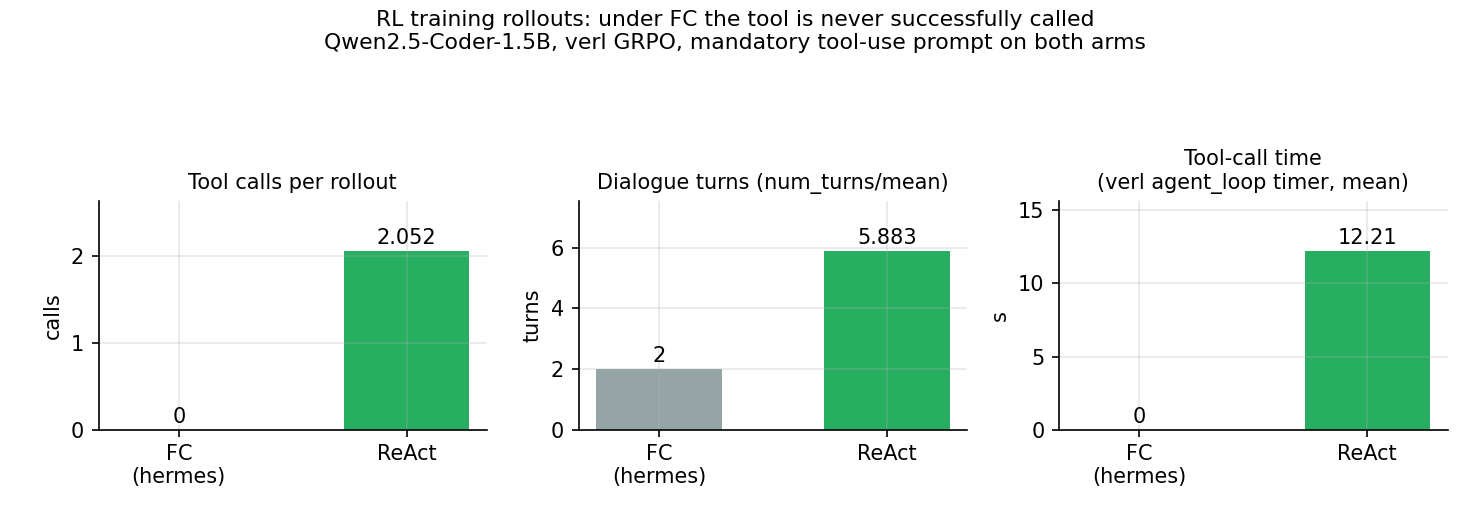
\includegraphics[width=\linewidth]{fig3_training_causal.png}
\caption{\textbf{Historical 1.5B RL diagnostic.} Under function calling the tool is never
successfully called; \texttt{num\_turns} stays pinned at its minimum of 2 and tool time is exactly
zero. Prompt strength is matched across arms (both mandatory); step counts are not (10 vs 3).
The formal 7B parser control is reported separately in Table~\ref{tab:p3formal}.}
\label{fig:train}
\end{figure}

\begin{center}
\small
\captionof{table}{Historical ReAct training with a working tool channel, 23{,}676 executed calls. Rescues by turn $\geq$2 do not move. The three historical 1.5B FC runs, in which \textbf{zero} tool calls executed, give rescue sequences $[7,9,6,6,7,6,10,8,9,8,6]$, $[8,7,6,7,7,7,7,5,6,6,8]$ and $[7,5,7,5,7,8,9,9,8,9]$. This is supporting evidence only; Table~\ref{tab:p3formal} is the single-variable control.}\label{tab:sufficiency}
\begin{tabular}{@{}lrrrr@{}}
\toprule
step & turn-1 & final & \textbf{rescued by turn $\geq$2} & repair channel \\
\midrule
0  & 359 & 367 & 8 & 263 \\
15 & 340 & 346 & \textbf{6} & 266 \\
30 & 340 & 346 & \textbf{6} & 262 \\
45 & 341 & 349 & \textbf{8} & 261 \\
60 & 341 & 347 & \textbf{6} & 274 \\
\bottomrule
\end{tabular}
\end{center}

\subsection{Sampling variance, and an inverted noise structure}
\label{sec:variance}

Llama-3.1-8B, \texttt{temperature=0.6}, n=100 $\times$ 3 seeds.

\begin{center}
\small
\captionof{table}{Sampling variance. FC seed 3 contains one rejected parallel-call request. We report its complete-denominator endpoint, and treat the two clean arms separately; an SD from two clean seeds would be too unstable to summarize variation reliably.}\label{tab:variance}
\begin{tabular}{@{}lllll@{}}
\toprule
& seed 1 & seed 2 & seed 3 & admissible \\
\midrule
ReAct turn-1 & 53 & 56 & 43 & 3/3 \\
ReAct final & 72 & 72 & 72 & 3/3 \\
FC turn-1 & 44 & 44 & 45 & --- \\
FC final & 62 & 66 & 57$^{\dagger}$ & \textbf{2 clean / 3 end-to-end} \\
\bottomrule
\end{tabular}
\end{center}

FC seed 3 contains one request error --- the model emitted parallel tool calls and vLLM returned
\emph{``This model only supports single tool-calls at once''}. The end-to-end endpoint therefore
retains that task as a failure and is 57/100; the prespecified clean-arm analysis excludes the seed
and reports [62, 66]. An SD can be computed from two clean seeds, but would be an unstable estimate,
so we do not use it to characterize sampling variation. Worst case among clean arms: ReAct's
lowest (72) versus FC's highest (66) = \textbf{+6}.

\textbf{Inverted noise structure.} ReAct's turn-1 varies widely (43--56, sd 6.8) while its final
converges; FC's turn-1 is nearly constant (44--45, sd 0.58) while its final disperses. The
mechanism is compensation in the rescue count --- 19 / 16 / \textbf{29}, largest where turn-1 was
worst --- and in all three seeds the count of ``passed at turn 1 but failed finally'' is
\textbf{0}: the repair loop is monotone. \textbf{The three identical finals are a coincidence of
totals, not identical item sets}, and sd = 0.00 must not be read as ``ReAct is perfectly
stable''.

\subsection{Multi-turn repair stabilises the total while its composition keeps moving}
\label{sec:composition}

Two independent observations show the same structure. \emph{Across sampling seeds}: ReAct's final
pass is 72 / 72 / 72 at \texttt{temperature=0.6}, yet the solved sets have pairwise Jaccard
0.71--0.80 --- 15--24 items differ. \emph{Across training steps}: between steps 15 and 30 of the
ReAct run, 85 of 542 first-turn completions changed verbatim and 6 items flipped outcome (3
gained, 3 lost), leaving turn-1 and final pass numerically identical (340 / 346 at both
checkpoints). The policy is demonstrably moving; the aggregate is not.

The common structure is that \textbf{the repair loop absorbs perturbation upstream of it}. Two
consequences follow. \emph{For measurement}, an aggregate pass rate is a \textbf{poor instrument
for detecting change in a multi-turn agent}: it is stabilised by the very mechanism under study,
and item-level set comparison detects movement the total conceals. We report both throughout, and
note that had we reported only totals we would have concluded --- twice, on two different axes ---
that nothing was happening. \emph{For deployment}, stability of the total under sampling noise is
a property practitioners want, it is contributed by the multi-turn loop rather than the base
policy, and it is invisible in single-turn evaluation. \textbf{Bound}: both observations are on
one model family and one task, the identical totals are in part coincidence, and we do not claim
the aggregate is invariant --- only that it is far less sensitive than its components.

\subsection{The training verifier: seams, audit, and planned fixes}
\label{app:verifier}

The GRPO reward is outcome-only: it extracts the last submitted program, runs the item's own
\texttt{pytest} suite in the sandbox, and returns the pass ratio (\texttt{reward\_code.py}). Three
reward-hacking routes are closed by construction --- a run in which no test executes scores 0
rather than 1, a timeout scores 0, and an item with no test string scores 0. The historical
verifier nevertheless had two seams. \emph{(i)} Its summary parser searched
\texttt{(\textbackslash d+) passed} over merged stdout/stderr and took the first match, so model
stdout could imitate pytest's summary. \emph{(ii)} \texttt{skipped} and \texttt{xfail} were not
counted in the denominator. Both were reachable in principle. We therefore audited:
across the five training logs that retain generated code there are \textbf{zero} occurrences of a
printed \texttt{``N passed''}, of \texttt{pytest.skip}/\texttt{allow\_module\_level}, or of
\texttt{sys.exit}/\texttt{os.\_exit}, and \texttt{critic/rewards/mean} oscillates in 0.46--0.73
without the step change a discovered exploit produces. The audit's own limit is that historical
full rollout text was not retained, so it covers only the fragments those logs carry. Before the
formal 7B control we anchored the regex to pytest's summary, included
\texttt{skipped}/\texttt{xfailed}/\texttt{xpassed} in the denominator, and retained every rollout
in full with a SHA-256 digest. Both P3 arms use this fixed verifier. Neither verifier path is used
for the reported held-out pass rates, which require \texttt{mode="script"}, a zero exit code and
\texttt{status=="ok"}.
